\section{Related Work}
\label{2017-coo-spmv:s2-related}

\begin{figure}[t]
\centering
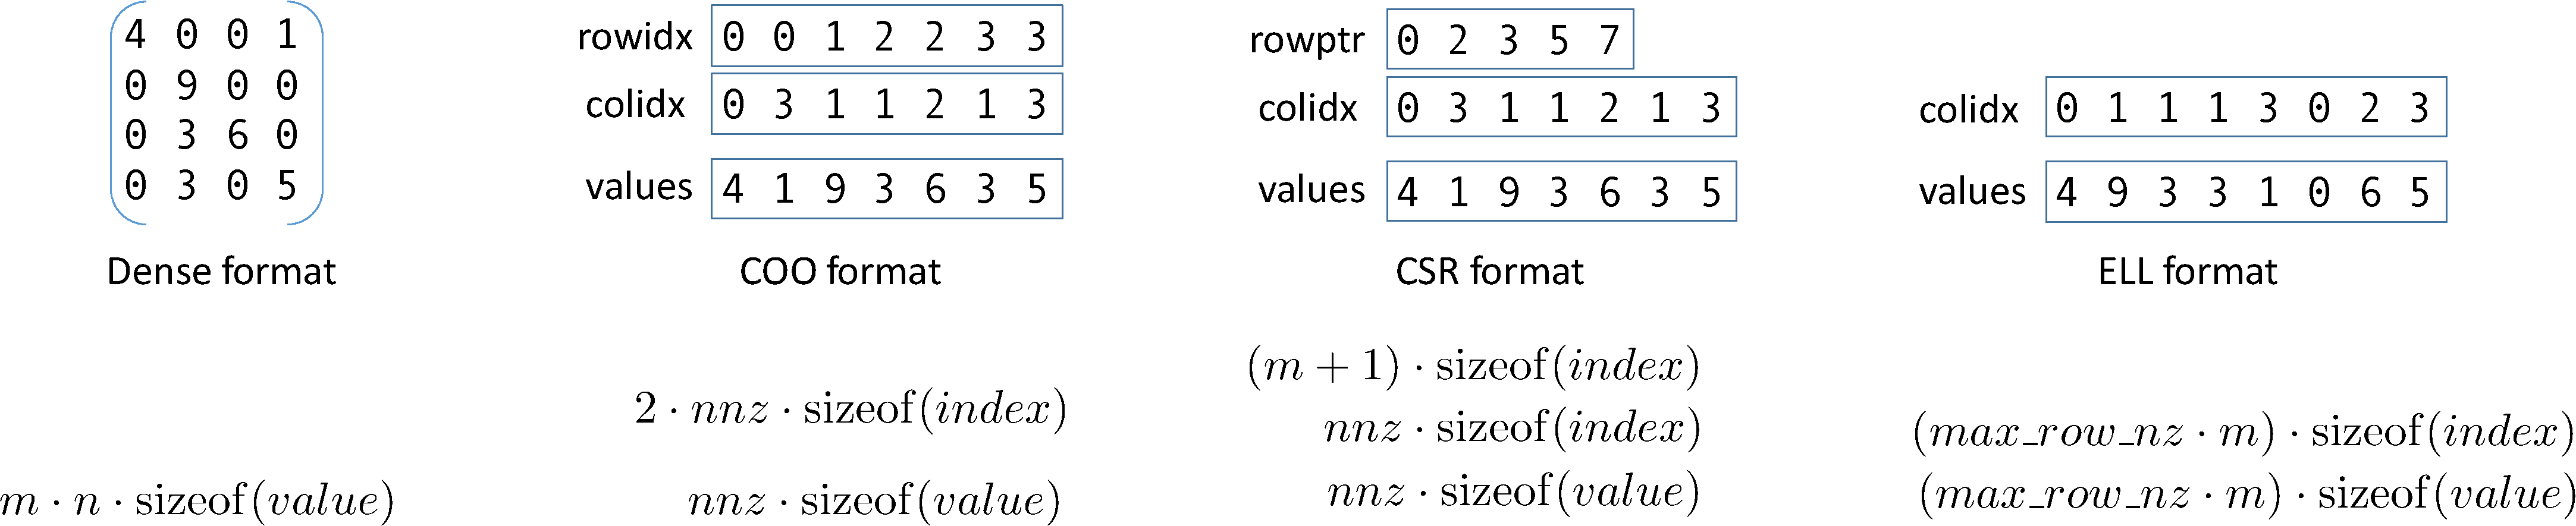
\includegraphics[width=\textwidth]{plots/formats}
\caption
[Different storage formats for a sparse matrix]
{Different storage formats for a sparse matrix of dimension $m\times n$
containing $nnz$ nonzeros along with the memory consumption.}
\label{2017-coo-spmv:fig:formatoverview}
\end{figure}

\subsection{Sparse Matrix Formats}
In the BLAS and LAPACK~\cite{lapack} standard for dense linear algebra, 
matrices are stored as a sequence of columns, with each column stored as an
array of its elements.
This allows to easily locate or identify any matrix entry in memory.
For matrices where most elements are zero, which is typical for, e.g., finite
element discretizations,
storing all matrix entries results in significant storage overhead.
The computational cost of a matrix vector product increases as well, as a result
of explicitly multiplying the zero entries with vector values.
Sparse matrix formats aim at reducing the memory footprint (and computational) 
cost by storing only the nonzero matrix values. Some formats additionally store
a moderate amount of zero elements to enable faster processing when computing
matrix vector products. Obviously, storing only a subset of the elements
requires to accompany these values with information that allows to deduce their
location in the original matrix.

A straight-forward idea is to explicitly store only the nonzero elements,
along with the row and column index of each element.
This storage format, known as coordinate (COO~\cite{barrettemplates}) format,
allows to determine the original position of any element
in the matrix without processing other entries.

Further reduction of the storage cost is possible if the elements are
sorted row-wise, and with increasing column-order in every row.
(The latter assumption is technically not required,
but it usually results in better performance.)
Then, the Compressed Sparse Row (CSR~\cite{barrettemplates}) format
can replace the array containing the row indexes with a pointer to the
beginning
of the distinct rows. While this reduces the data volume,
the CSR format requires extra processing to determine the row location of
a certain element.

On SIMD architectures, a performance-relevant aspect is to have uniform operations
across the SIMD unit. This makes the ELL format~\cite{ellpack} attractive for these architectures:
In this format, each row is compressed to contain only the nonzero entries 
and some explicit zeros that are used for padding to enforce
an equal length for all rows.
The resulting value matrix is accompanied with a column index matrix which stores
the column position of each entry in the compressed matrix.
While typically increasing the storage cost compared to the CSR format,
this removes the need for explicitly storing the row pointers.
Furthermore, the column indexes (and values) in the distinct
rows can be processed in SIMD fashion.
Coalescent (SIMD-friendly) memory access is enabled if the value and column
index matrices are stored in column-major order.

To reduce the memory overhead, the ELL format can be truncated to a version
where only row-blocks with the height of the SIMD-length are padded to the
same number of nonzero elements, but the rows in distinct blocks can differ in
the number of nonzero elements.
This ``sliced ELL'' (SELL-p~\cite{sellcs}) format can be viewed as splitting the matrix into row-blocks
and storing each block in ELL format.
The formats discussed in this section are visualized
in Figure~\ref{2017-coo-spmv:fig:formatoverview}.

Aside from these basic formats, there exist variants
which arise as combinations of these basic formats:
e.g., the hybrid format which stores the matrix partly in ELL and partly in
CSR or COO.


\subsection{SpMV on manycore architectures}

Related to the storage format is the question of how to process
the multiplication with a vector in parallel.
The main challenges in this context are: 
1) balancing the workload among the distinct cores/threads; and 
2) allowing for efficient access to the matrix entries and the vector values.
The second aspect is relevant in particular on NVIDIA GPUs where each memory access
reads 128 contiguous bytes of memory~\cite{cuda8.0}.
In case of fine-grained parallelism, balancing the workload naturally results in 
multiple threads computing partial sums for one row, which requires careful synchronization
when writing the resulting vector entry back into main memory.

The standard approach of parallelizing the CSR, ELL and SELL-p formats is to
distribute the rows among distinct threads (or groups of threads)
\cite{ellpack, sellc}.
For the CSR format, this works fair well for balanced sparsity patterns, but it can lead to
severe load imbalance otherwise. 
Recently, a strategy for a load balanced CSR \spmv was proposed that 
parallelizes across the nonzero elements instead the rows~\cite{csri}. 
The \spmv kernel we present in this paper is based on the COO format, which 
comes with the advantage of the row index of an element being readily available.
